\chapter{Multichannel Acoustic Pulse Recognition System}\label{ch:MultichannelAPR}

\ifpdf
    \graphicspath{{Chapter4_MultiAPR/Chapter4Figs/PNG/}{Chapter4_MultiAPR/Chapter4Figs/PDF/}{Chapter4_MultiAPR/Chapter4Figs/}{Chapter4_MultiAPR/Chapter4Figs/Training/}}
\else
    \graphicspath{{Chapter4_MultiAPR/Chapter4Figs/EPS/}{Chapter4_MultiAPR/Chapter4Figs/}}
\fi

%Introduction to multichannel APR
While a key aspect of the basic single channel Acoustic Pulse Recognition (APR) system was founded in the breath of devices in the market meeting the hardware requirements for the system presented in chapter~\ref{ch:APR}, a range of devices are emerging with multiple sensors, and specifically multiple microphones. Laptop computers, tablets and mobile phones frequently employ multiple microphones for noise cancellation\cite{Habets2013}\cite{Habets2012}, echo cancelation\cite{US7925007} and localisation applications\cite{US8174547}\cite{US8233353}.

In this chapter the APR system is generalised to multiple channels and results are provided to quantify the multi channel APR system's performance in relation to a single channel equivalent.

%outline of chapter
\todo{outline of chapter}

\section{Background}
%Discuss and outline the advantages of multiple channels in a physical detection application
Chapter~\ref{ch:APR} described the theory and application of a single channel APR system. This system relied on the existence of a single transducer in or on the device for the APR application. For many devices this microphone implementation would be designed for speech recordings and design specifications may have included steps to actively reduce the impact of mechanically noise in the device. Multiple channels enables theoretically improved performance on two accounts. Firstly since the channels can be considered parallel and independent, each additional channel may be considered an independent trial with same results. This is particularly an advantage when the additional available channels are designed to specifically be a reference source discounting either some noise source (say background noise) or the target source (say speech). This enables a secondary detection or classification channel potentially affected to a lesser extent by either speech or other noise.

\subsection{Time of Flight (ToF)}
A second advantage of the multi channel system is the main functional component of previous multichannel APR systems\cite{TouchSystems2006}\cite{US7411581}. Time of Flight (ToF) or Time Delay of Arrival (TDA) or the relative time of arrival of especially transient events at uniquely placed receiving transducers gives an additional indication of the origin of a pulse.

Consider a tap on a surface which generates a pulse and thereby an acoustic wavefront propagating radially outwards from the point of impact. The array of microphones embedded in the surface will receive the wavefront at different times relative to their distance from the point of impact and the phase velocity. Figure~\ref{fig:ToFexample.pdf} shows an example of a surface with a wavefront's propagation and 3 microphones' relative position within the propagation pattern.

\begin{figure} %ToFexample.pdf
\begin{minipage}[b]{1.0\linewidth}
  \centering
  \centerline{\includegraphics[width=12cm]{ToFexample.pdf}
  \begin{picture}(0,0)
\put(-200,5){Microphone}
\put(-310,5){Impact site}
\put(-80,5){Wavefront}
\end{picture}}
\end{minipage}
\caption{An example of a wavefront's radial propagation in a surface and 3 embedded microphones. All reflections are omitted.}
\label{fig:ToFexample.pdf}
\end{figure}

No timing or localisation information can be inferred from a single microphone where as a set of microphones provide a hyperbolic curve upon which the event must have occurred. No less than 3 microphones are required to locate the origin of a tap on a 2 dimensional plane\cite{US7411581}. %Figure~\ref{fig:MultiSourceExample.pdf}(a) and (b) provides an example of 3 waveforms from 3 different microphones located a different points in a system.

%Discuss time of flight (ToF) (and sample rates/size tradeoff)
For constant phase speed $c$ in a specific material and time difference $\Delta t$ the spatial difference between microphones $\Delta d$ can be calculated with a basic equation of motion,

\begin{equation}\label{eq:ToFcalcs1}
\Delta d  = c \Delta t.
\end{equation}

For a digital system sampled at sampling rate $f_s$, time difference is equivalent to $\Delta t = \Delta S/f_s$ where $S$ is the a number of samples and $t$ and sampling rate is measured in seconds and samples per second respectively.

The positional difference $\Delta d$ can now be calculated from the sample difference $\Delta S$ between two events as,

\begin{equation}\label{eq:ToFcalcs2}
\Delta d  = c \frac{\Delta S}{f_s}.
\end{equation}

For the minimum sampling rate $f_s$ needed to detect any spatial difference $\Delta S \leq 1$ equation~\ref{eq:ToFcalcs2} is rearranged to

\begin{equation}\label{eq:ToFcalcs3}
f_s  \geq \frac{c}{\Delta d}.
\end{equation}

Figure~\ref{fig:MultiSourceExampleAnnoSpot9.pdf} shows an example of 3 waveforms from 3 different microphones embedded in a surface. Various points on the waveforms have been affixed with data tags to allow for a comparison of their relative arrival times. In this example the absolute distant in the surface from the microphones to the impact site was 30, 10 and 20 cm for microphones 1, 2 and 3 respectively. It is important to note that so far it has been the first arrivals that have been of primary concern for the positioning of signals, but Figure~\ref{fig:MultiSourceExampleAnnoSpot9.pdf} also shows other waveform elements related to the surface geometry. Microphone 3 provides a clear secondary negative peak at sample number 45. This secondary peak quite likely corresponds to a reflected (non direct) pulse arriving slightly delayed to the direct pulse due to the longer path travelled.

\begin{figure} %MultiSourceExampleAnnoSpot9.pdf
\begin{minipage}[b]{1.0\linewidth}
  \centering
  \centerline{\includegraphics[width=12cm]{MultiSourceExampleAnnoSpot9.pdf}
  \begin{picture}(0,0)
\put(-180,60){11}
\put(-150,36){19}
\end{picture}}
\end{minipage}
\caption{A zoomed example of the 3 wavefronts captured, and their relative alignment, for an impact on spot 9 on the surface.}
\label{fig:MultiSourceExampleAnnoSpot9.pdf}
\end{figure}

Based on the estimated phase speed in the surface, provided in appendix~\ref{ap:SpeedCalc}, this additional distance is 4.4 cm approximately corresponding to a range of early reflective paths on the surface.


\section{Model and theory}\label{sec:MultiAPRModelTheory}
The multi channel model proposed here is an extension of the multi component model proposed in section~\ref{sec:APRpca}.

Similarly to equation~\ref{eq:mod1} we consider observations of the form $y_c = [y_{c,0}, \ldots , y_{c,N-1}]^T$ for the $c$th channel so that $\textbf{y} = [y_c, \ldots, y_C]$ for $C$ independent channels. The standard noisy linear instantaneous model is considered for a single channel $c$:

\begin{equation}\label{eq:mod1_c}
y_c = \sum_{i=1}^{I} \theta_{c,i}^j t_{c,i}^j(n_0) + v_c,
\end{equation}

where $t_{c,i}^j(n_0)$ is the $j$th template for the $c$th channel, $j_c \in \{1, \ldots ,J\}$, for $I$ independent components and $\theta_{c,i}^j$ is the amplitude of the $c$th channel, $j$th spot and $i$th component. In this section the model has been assumed to be of zero mean $\mu_c^j(n_0) =0$ although this assumption could easily be avoided by adding it to the model. Take $\theta_{c,i}^j$ to be a random variable, $\Theta_c^j = [\theta_{c,1}^j,\ldots,\theta_{c,I}^j]^T$, describing the scale of each template component $i$ where

\begin{equation}\label{eq:theta_c}
\Theta_c^j \sim \mathcal{N}(\mu_{\Theta_c}^j,C_{\Theta_c}^j),
\end{equation}

and Gaussian noise to model background interference:

\begin{equation}\label{eq:noise_c}
v_{c,n} \stackrel{i.i.d.}{\sim} \mathcal{N}(0,\sigma_{v,c,n}^2).
\end{equation}

Considering this model in matrix notation:
\begin{equation}\label{eq:mod2}
y_c = \textbf{t}_c\Theta_c + \textbf{v}_c.
\end{equation}

Bayes' theorem can now be used to evaluate the joint probability of $\textbf{y}$ and $\Theta$ as

\begin{equation}\label{eq:bayes1_c}
p(\textbf{y},\Theta | j, c) = p(\textbf{y}|\Theta,j,c)p(\Theta | j,c).
\end{equation}

Since the goal is to evaluate the probability of each data reading $\textbf{y}$ given a particular position/model $j$, the dependency of $\Theta$ can be marginalized out,

\begin{eqnarray}\nonumber
p(\textbf{y}|j) &=& \int_\Theta p(\textbf{y},\Theta|j) d\Theta \\
\label{eq:marg1_c} &=& \int_\Theta p(\textbf{y}|\Theta,j)p(\Theta|j) d\Theta.
\end{eqnarray}

As with the single channel method, see equation~\ref{eq:loglikeli}, the log-likelihood is calculated

\begin{equation}\label{eq:loglikeli_c}
\log{p(y_c|j)} = - \frac{n}{2}\log{2 \pi}- \frac{1}{2}\log{|\Phi_c|} - \frac{1}{2}\log{|C_{\Theta,c}|} - \frac{1}{2\sigma^2_{v,c}}\left(\sigma_{v,c}^2\mu_\Theta^TC_{\Theta,c}^{-1}\mu_{\Theta,c} + y_c^Ty_c- \left(\Phi_c^T\right)^{-1}\Lambda_c^T\Lambda_c\right).
\end{equation}

Since the channels are considered independent of each other we have that

\begin{equation}\label{eq:jointprob_c}
p(\textbf{y} | j) = \prod^C p(\textbf{y} | j, c).
\end{equation}

Similar to equation~\ref{eq:MLdefinition}, the Maximum Likelihood estimator can be expressed as

\begin{equation}\label{eq:MLdefinition_c}
p(j |\textbf{y}) = \argmax{j} \prod^C p(y|j,n_0,c),
\end{equation}

\begin{equation}\label{eq:MLdefinition_c}
\log{\left( p(j |\textbf{y})\right)} = \argmax{j} \sum^C \log{\left( p(y|j,n_0,c) \right)}.
\end{equation}

\section{Training}\label{sec:MultiAPRTraining}
%describe the different training schemes employed
The training of the templates for the multi channel APR system proceeds similarly to the single channel APR PCA based system outlined in section~\ref{sec:APRtraining} with a few exceptions. In this chapter 4 different methods will be compared, while these will be described in detail in section~\ref{sec:MultiAPRMethod}, the training for these models will be outlined below.

The diagram presented in Figure~\ref{fig:trainingSystem1.pdf} outlines the most basic, or the base line approach that will be tested in this chapter. Each channel $c$ will be considered independently and so the training stage will exactly mirror that presented in section~\ref{sec:MultiAPRMethod} relating to the PCA training with $J$ different templates.

\begin{figure} %trainingSystem1.pdf
\begin{minipage}[b]{1.0\linewidth}
  \centering
  \centerline{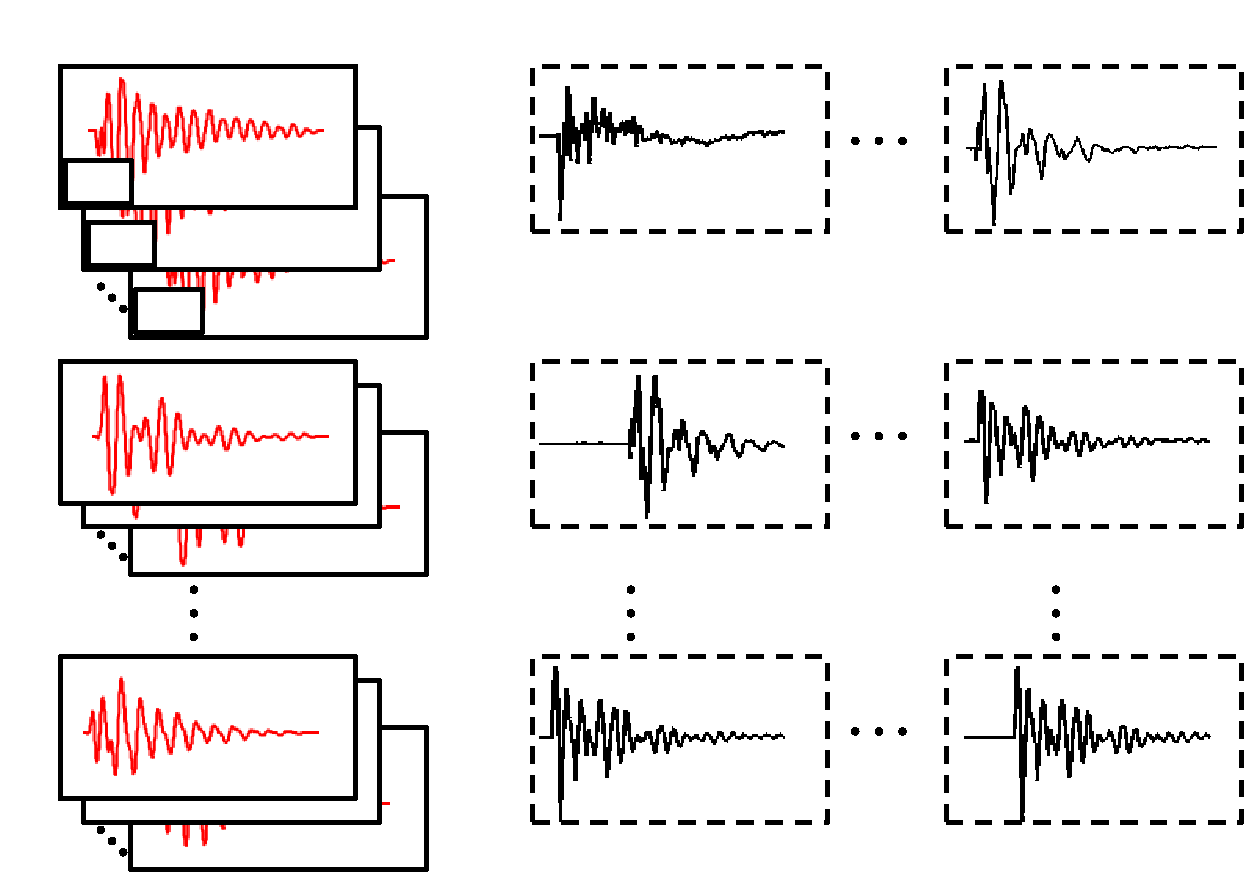
\includegraphics[width=13cm]{trainingSystem1.pdf}
  \begin{picture}(0,0)
  \put(-334,255){Training}
  \put(-133,255){Testing}
\put(-351,205){j=1}
\put(-344,187){j=2}
\put(-329,167){j=J}
\put(-380,219){c=1}
\put(-380,129){c=2}
\put(-380,41){c=C}
\end{picture}}
\end{minipage}
\caption{Example of individual training per channel $c$ and the templates' application in testing.}
\label{fig:trainingSystem1.pdf}
\end{figure}

An initial implementation of the multichannel system training is shown in Figure~\ref{fig:trainingSystem2.pdf}. Here the templates are considered together but aligned independently. This approach follows the training method presented in section~\ref{sec:MultiAPRMethod} and while the classification probabilities are considered jointly the templates are trained independently allowing for different templates with different lengths and number of components.

\begin{figure} %trainingSystem2.pdf
\begin{minipage}[b]{1.0\linewidth}
  \centering
  \centerline{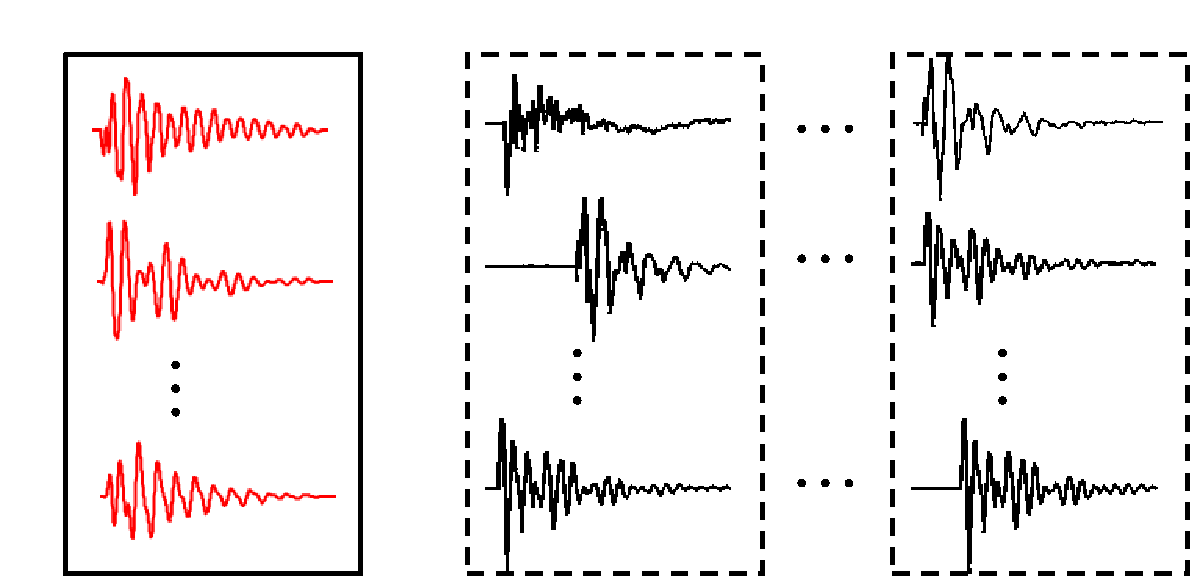
\includegraphics[width=13cm]{trainingSystem2.pdf}
  \begin{picture}(0,0)
    \put(-334,220){Training}
  \put(-137,220){Testing}
\put(-351,50){j=1}
\put(-342,33){j=2}
\put(-334,9){j=J}
\put(-380,180){c=1}
\put(-380,133){c=2}
\put(-380,65){c=C}
\end{picture}}
\end{minipage}
\caption{Example of individually aligned training but joint probability, and the templates' application in testing.}
\label{fig:trainingSystem2.pdf}
\end{figure}

Figure~\ref{fig:trainingSystem3.pdf} shows the multi channel APR system training using joint alignment. While, as in section~\ref{sec:MultiAPRMethod}, the other methods presented here have trained each channel independently, this approach only prompts the trainer for alignment cues based on data from one channel. This means that the relative alignments between channels $c$ and spots $j$ remain intact. Data associated with each channel can be stored independently as previously but each template will now be of similar length and will require slightly longer templates to account for impulses arriving prior to those of the alignment channel (channel 1 $c=1$ for all tests conducted).

\begin{figure} %trainingSystem3.pdf
\begin{minipage}[b]{1.0\linewidth}
  \centering
  \centerline{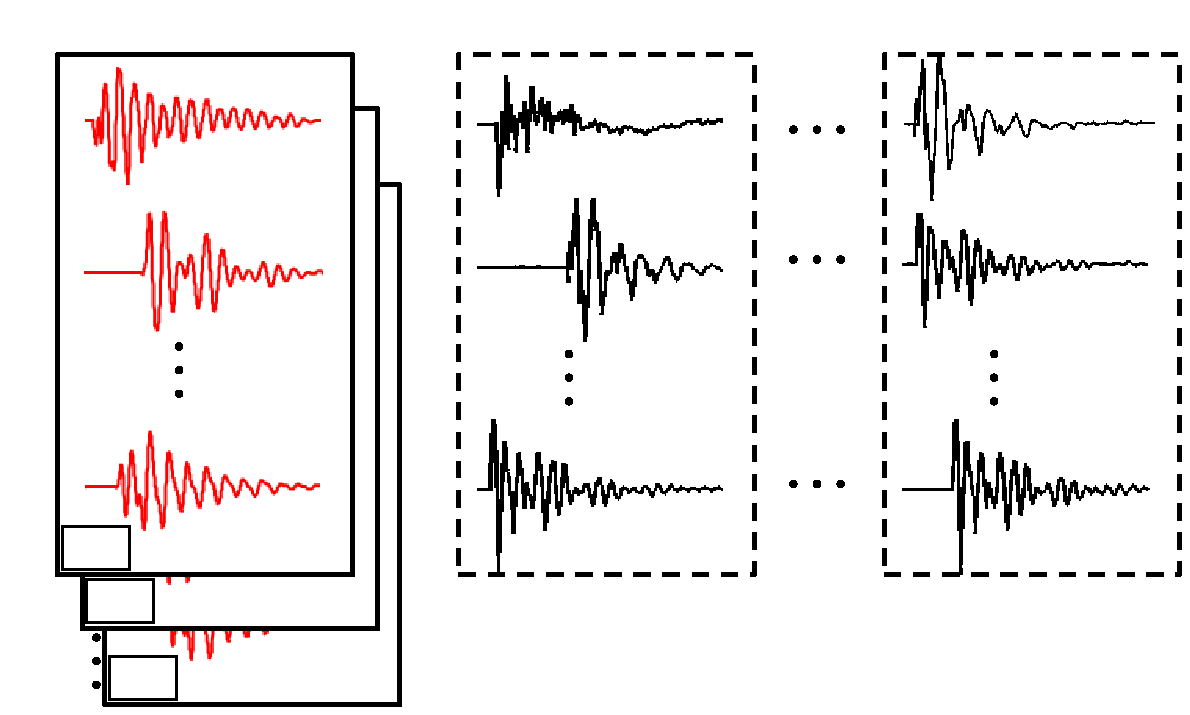
\includegraphics[width=13cm]{trainingSystem3.pdf}
  \begin{picture}(0,0)
    \put(-334,220){Training}
  \put(-137,220){Testing}
\put(-350,49.5){j=1}
\put(-342,33){j=2}
\put(-334,9){j=J}
\put(-380,182){c=1}
\put(-380,135){c=2}
\put(-380,68){c=C}
\end{picture}}
\end{minipage}
\caption{Example of fixed alignment training, and the templates' application in testing.}
\label{fig:trainingSystem3.pdf}
\end{figure}

\section{Method}\label{sec:MultiAPRMethod}



\subsection{System setup}\label{sec:MultiAPRSystem}
%tests Q for q=1 to q=Q

\begin{figure} %MultiAPRsystem.pdf
\begin{minipage}[b]{1.0\linewidth}
  \centering
  \centerline{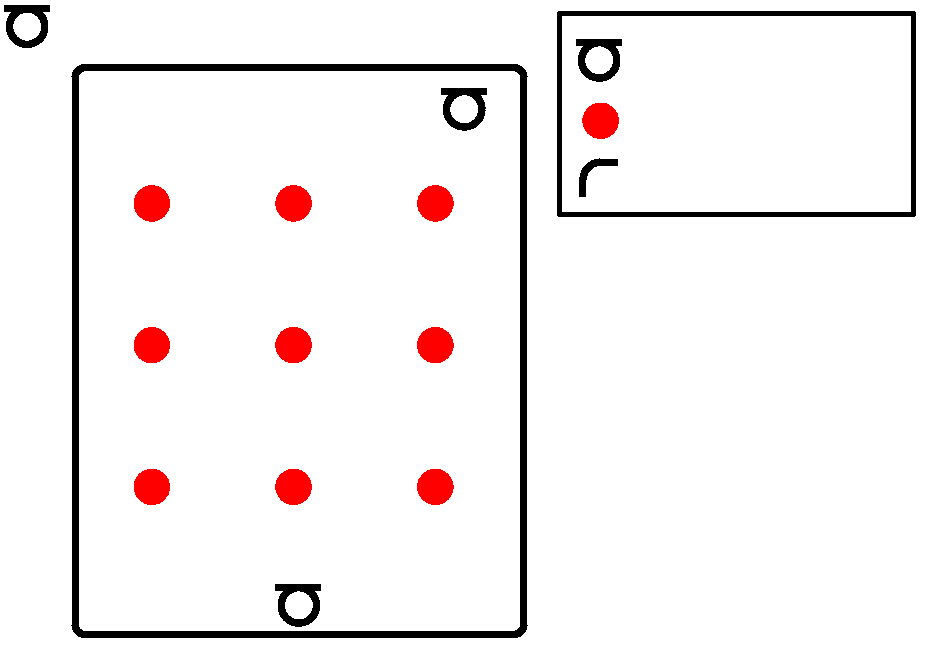
\includegraphics[width=10cm]{MultiAPRsystem.pdf}
  \begin{picture}(0,0)
\put(-90,176){Microphone}
\put(-90,158){Impact site}
\put(-90,140){Surface edge}
\end{picture}}
\end{minipage}
\caption{}
\label{fig:MultiAPRsystem.pdf}
\end{figure}

\subsection{Approaches}
While the underlying theory behind the multi channel APR system was outlined in section~\ref{sec:MultiAPRModelTheory}, the actual implementation of decision process can be approached in various ways. This section will outline the ones for which training approaches were presented in section~\ref{sec:MultiAPRTraining} and results are presented in section~\ref{sec:MultiAPRResults}.

As mentioned previously the multi channel approach will be compared to the standard single channel approach. The single channel PCA method will be run for each channel $c$ and will return a total number of $QC$ results for $Q$ tests and $C$ channels as shown in Figure~{fig:trainingSystem1.pdf}. In addition the single channel results will be processed and the unique mode for each test $q$ result, if it exists, will be shown together with the median for each test $q$.

    


\section{Results}\label{sec:MultiAPRResults}
\subsection{ToF example}
\begin{figure} %MultiSourceExample.pdf
\begin{minipage}[b]{1.0\linewidth}
  \centering
  \centerline{\includegraphics[width=12cm]{MultiSourceExample.pdf}
  \begin{picture}(0,0)
\put(-320,360){(a)}
\put(-320,168){(b)}
\end{picture}}
\end{minipage}
\caption{(a) An example of the 3 wavefronts captured, and their relative alignment, for an impact on spot 9 on the surface. (b) Zoomed in version of (a).}
\label{fig:MultiSourceExample.pdf}
\end{figure}

\section{Discussion}
\section{Conclusions}

%Further work
%correlate noise
%Correlate \theta in a channel internally

% ------------------------------------------------------------------------


%%% Local Variables:
%%% mode: latex
%%% TeX-master: "../thesis"
%%% End:
